Here’s the complete code for our Alloy model. The .als file can be found in our
GitHub repository. For clarity we separate the code in Signatures, Facts and
Asserts and Predicates.

\subsection{Abstract Entity and Signature}
%%you cna use this command to import code written in .als to the latex file

\lstinputlisting[language=alloy]{Alloy/Model3.als}

\subsection{Worlds Generated}
Here are presented one generated world using the Alloy verification software. The diagram is the predicate show() for 2 cases.
The generated world represents the situation where a registered user has reported a violation. The photo taken by the user sent to the ALPR entity which is responsible to extract the license plate and return the extracted license plate to the Violation entity. Authority and EndUsers are also able to access to the Mined information according to their privileges. In our scenario an Authority is allowed to access both mined offender and mined streets information but an end user can only be able to access to mined street information. Another things to notice is that a ticket issue for a violation if and only if it is true and be approved by the authority.

\begin{figure}[H]
		\centering
      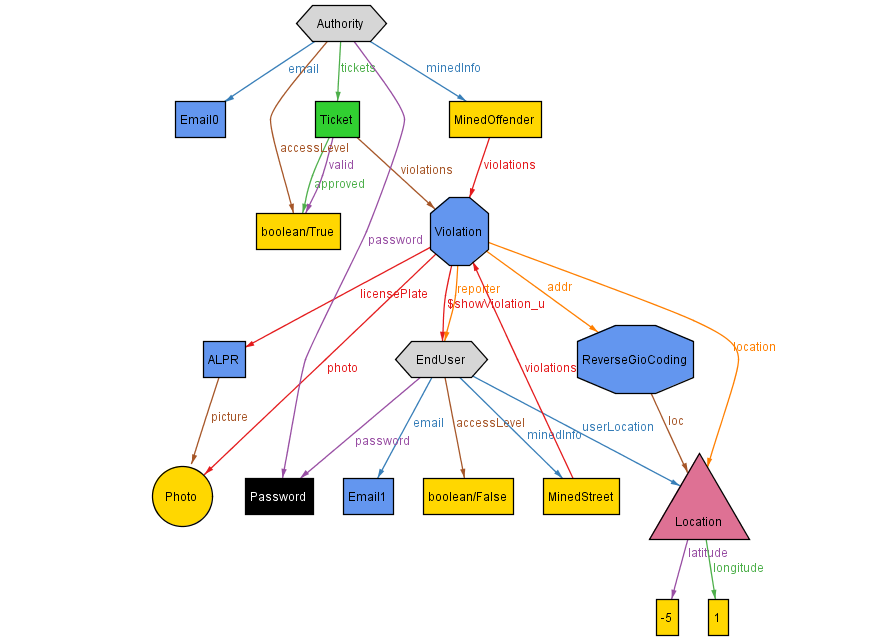
\includegraphics[width=0.5\textwidth]{Images/alloy.PNG}
      \caption{Alloy Model 1}   \label{fig:alloy}
\end{figure}
